\documentclass{standalone}
\usepackage{tikz}
\usetikzlibrary{patterns, positioning}
\usepackage[sfdefault]{ClearSans} %% option 'sfdefault' activates Clear Sans as the default text font
\usepackage[T1]{fontenc}

\begin{document}
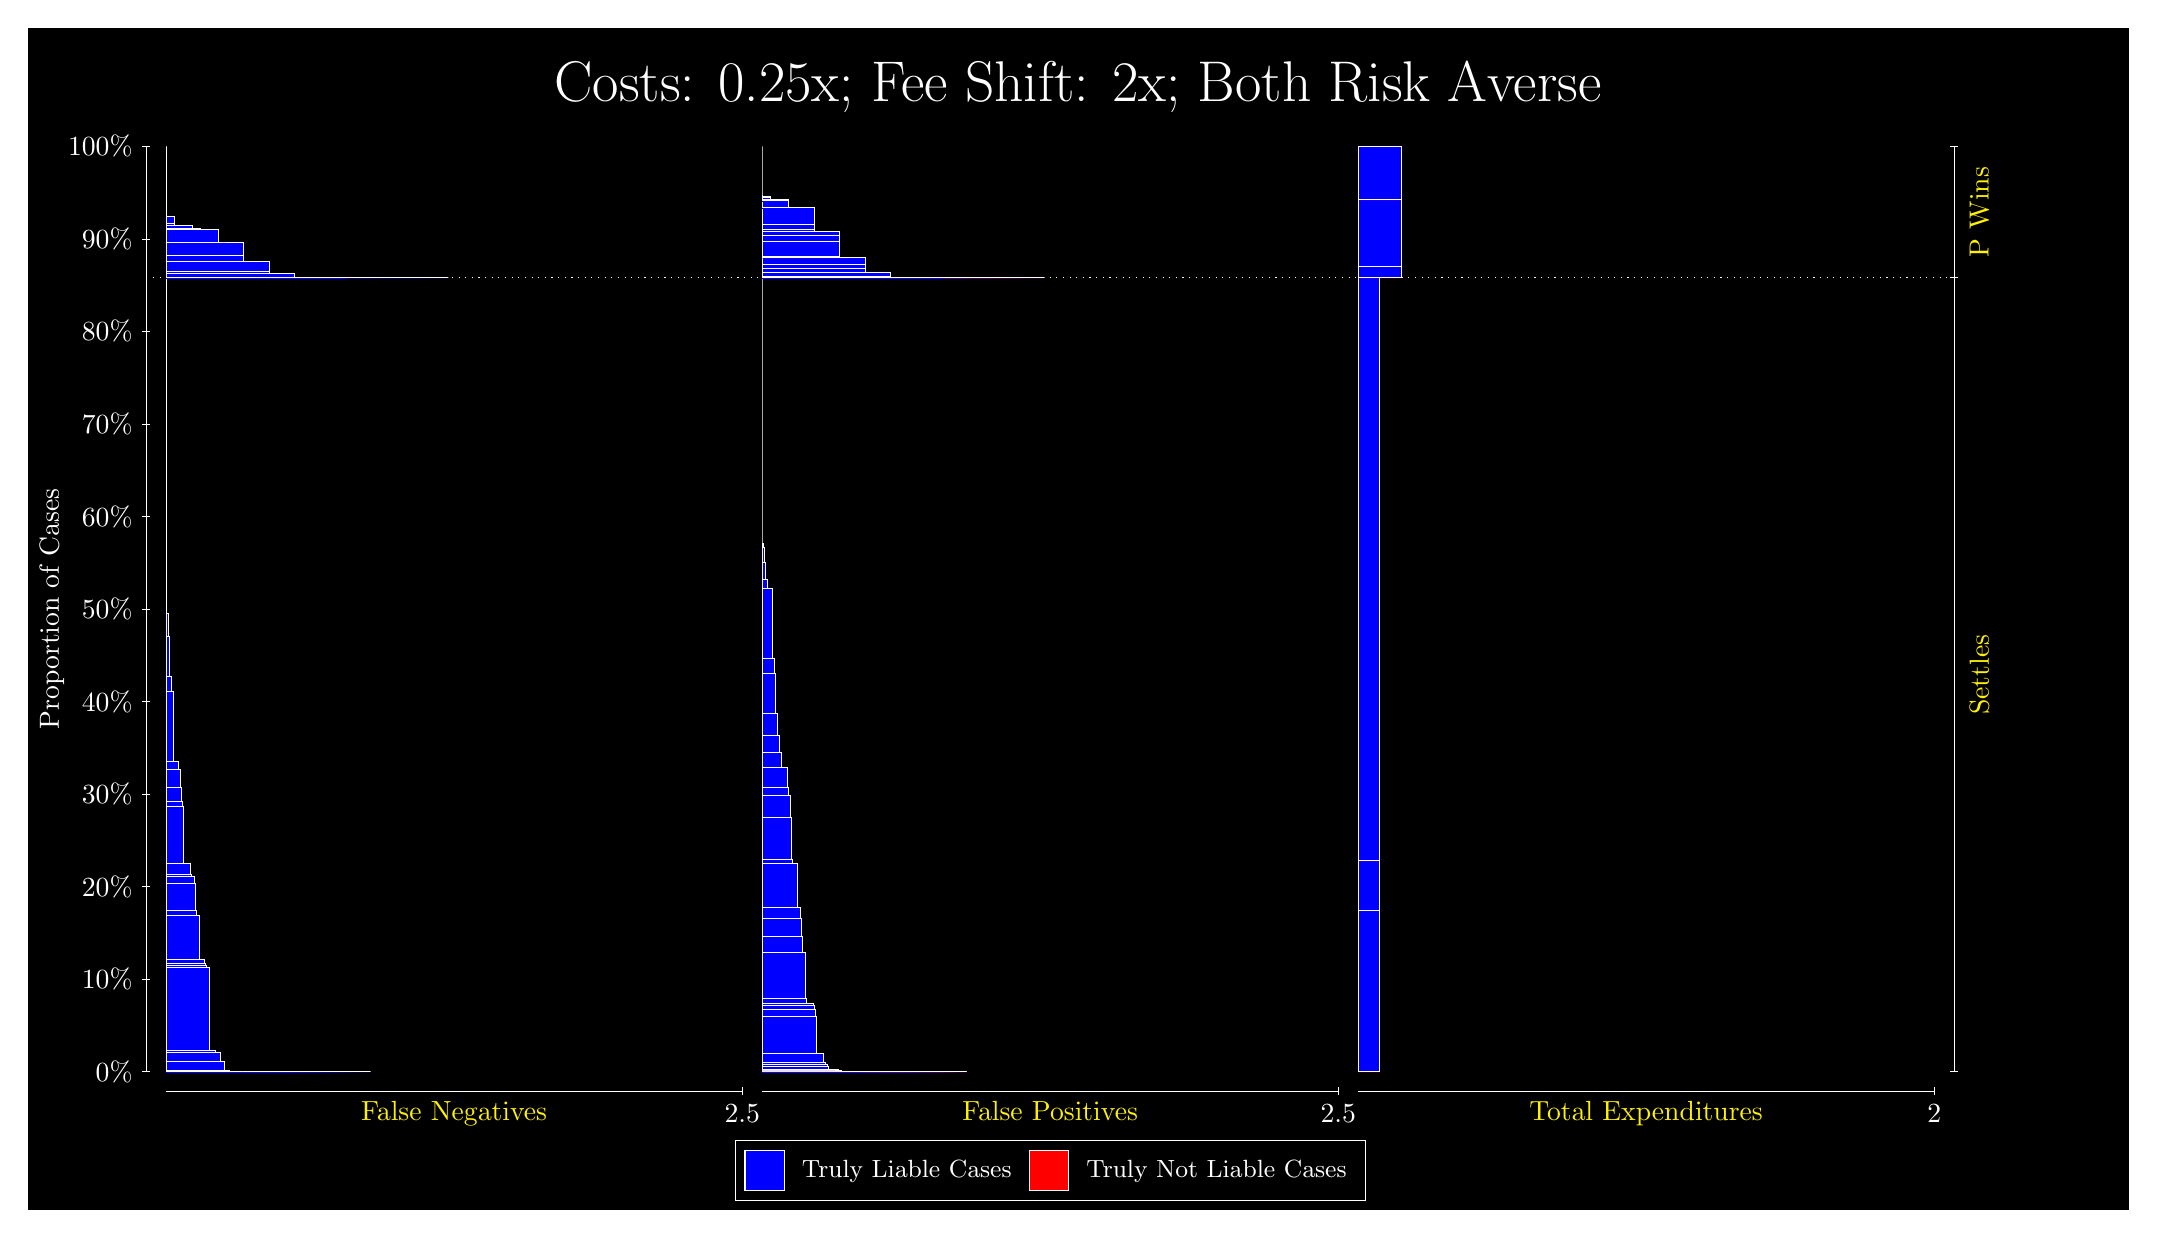
\begin{tikzpicture}
\draw[fill=black] (0,0) rectangle (26.667,15);
\draw[text=white] (0,13.5) rectangle (26.667,15) node[midway] {\huge Costs: 0.25x; Fee Shift: 2x; Both Risk Averse};
\draw[white, very thin] (1.5,1.75) -- (1.5,13.5);
\node[rotate=90, text=white, anchor=center] at (0.3, 7.625) {Proportion of Cases};
\draw[white, very thin] (1.45,1.75) -- (1.55,1.75);
\node[text=white, anchor=east] at (1.45, 1.75) {0\%};
\draw[white, very thin] (1.45,2.925) -- (1.55,2.925);
\node[text=white, anchor=east] at (1.45, 2.925) {10\%};
\draw[white, very thin] (1.45,4.1) -- (1.55,4.1);
\node[text=white, anchor=east] at (1.45, 4.1) {20\%};
\draw[white, very thin] (1.45,5.275) -- (1.55,5.275);
\node[text=white, anchor=east] at (1.45, 5.275) {30\%};
\draw[white, very thin] (1.45,6.45) -- (1.55,6.45);
\node[text=white, anchor=east] at (1.45, 6.45) {40\%};
\draw[white, very thin] (1.45,7.625) -- (1.55,7.625);
\node[text=white, anchor=east] at (1.45, 7.625) {50\%};
\draw[white, very thin] (1.45,8.8) -- (1.55,8.8);
\node[text=white, anchor=east] at (1.45, 8.8) {60\%};
\draw[white, very thin] (1.45,9.975) -- (1.55,9.975);
\node[text=white, anchor=east] at (1.45, 9.975) {70\%};
\draw[white, very thin] (1.45,11.15) -- (1.55,11.15);
\node[text=white, anchor=east] at (1.45, 11.15) {80\%};
\draw[white, very thin] (1.45,12.325) -- (1.55,12.325);
\node[text=white, anchor=east] at (1.45, 12.325) {90\%};
\draw[white, very thin] (1.45,13.5) -- (1.55,13.5);
\node[text=white, anchor=east] at (1.45, 13.5) {100\%};

\draw[white, very thin] (24.457,1.75) -- (24.457,13.5);
\draw[white, very thin] (24.407,1.75) -- (24.507,1.75);
\node[anchor=west] at (24.407, 1.75) {};
\draw[white, very thin] (24.407,11.831) -- (24.507,11.831);
\node[anchor=west] at (24.407, 11.831) {};
\draw[white, very thin] (24.407,13.5) -- (24.507,13.5);
\node[anchor=west] at (24.407, 13.5) {};

\draw[white, very thin, fill=blue] (1.75,1.75) rectangle (4.3482,1.75);
\draw[white, very thin, fill=blue] (1.75,1.75) rectangle (4.2018,1.75);
\draw[white, very thin, fill=blue] (1.75,1.75) rectangle (4.0554,1.75);
\draw[white, very thin, fill=blue] (1.75,1.75) rectangle (4.0229,1.75);
\draw[white, very thin, fill=blue] (1.75,1.75) rectangle (3.9091,1.75);
\draw[white, very thin, fill=blue] (1.75,1.75) rectangle (3.8765,1.75);
\draw[white, very thin, fill=blue] (1.75,1.75) rectangle (3.7627,1.75);
\draw[white, very thin, fill=blue] (1.75,1.75) rectangle (3.7302,1.75);
\draw[white, very thin, fill=blue] (1.75,1.75) rectangle (3.6976,1.75);
\draw[white, very thin, fill=blue] (1.75,1.75) rectangle (3.5838,1.75);
\draw[white, very thin, fill=blue] (1.75,1.75) rectangle (3.5513,1.75);
\draw[white, very thin, fill=blue] (1.75,1.75) rectangle (3.4699,1.75);
\draw[white, very thin, fill=blue] (1.75,1.75) rectangle (3.4374,1.75);
\draw[white, very thin, fill=blue] (1.75,1.75) rectangle (3.4049,1.75);
\draw[white, very thin, fill=blue] (1.75,1.75) rectangle (3.3723,1.75);
\draw[white, very thin, fill=blue] (1.75,1.75) rectangle (3.3236,1.75);
\draw[white, very thin, fill=blue] (1.75,1.75) rectangle (3.2585,1.75);
\draw[white, very thin, fill=blue] (1.75,1.75) rectangle (3.226,1.75);
\draw[white, very thin, fill=blue] (1.75,1.75) rectangle (3.1772,1.75);
\draw[white, very thin, fill=blue] (1.75,1.75) rectangle (3.1447,1.7501);
\draw[white, very thin, fill=blue] (1.75,1.7501) rectangle (3.1121,1.7501);
\draw[white, very thin, fill=blue] (1.75,1.7501) rectangle (3.0796,1.7501);
\draw[white, very thin, fill=blue] (1.75,1.7501) rectangle (3.0471,1.7501);
\draw[white, very thin, fill=blue] (1.75,1.7501) rectangle (3.0308,1.7501);
\draw[white, very thin, fill=blue] (1.75,1.7501) rectangle (2.9983,1.7501);
\draw[white, very thin, fill=blue] (1.75,1.7501) rectangle (2.9332,1.7501);
\draw[white, very thin, fill=blue] (1.75,1.7501) rectangle (2.9007,1.7501);
\draw[white, very thin, fill=blue] (1.75,1.7501) rectangle (2.8844,1.7505);
\draw[white, very thin, fill=blue] (1.75,1.7505) rectangle (2.8519,1.7505);
\draw[white, very thin, fill=blue] (1.75,1.7505) rectangle (2.8194,1.7558);
\draw[white, very thin, fill=blue] (1.75,1.7558) rectangle (2.7868,1.7558);
\draw[white, very thin, fill=blue] (1.75,1.7558) rectangle (2.7543,1.7559);
\draw[white, very thin, fill=blue] (1.75,1.7559) rectangle (2.7218,1.7559);
\draw[white, very thin, fill=blue] (1.75,1.7559) rectangle (2.7055,1.7564);
\draw[white, very thin, fill=blue] (1.75,1.7564) rectangle (2.673,1.7564);
\draw[white, very thin, fill=blue] (1.75,1.7564) rectangle (2.6079,1.7566);
\draw[white, very thin, fill=blue] (1.75,1.7566) rectangle (2.5917,1.7576);
\draw[white, very thin, fill=blue] (1.75,1.7576) rectangle (2.5754,1.758);
\draw[white, very thin, fill=blue] (1.75,1.758) rectangle (2.5591,1.7653);
\draw[white, very thin, fill=blue] (1.75,1.7653) rectangle (2.5266,1.7653);
\draw[white, very thin, fill=blue] (1.75,1.7653) rectangle (2.4941,1.877);
\draw[white, very thin, fill=blue] (1.75,1.877) rectangle (2.4616,1.8819);
\draw[white, very thin, fill=blue] (1.75,1.8819) rectangle (2.4453,1.994);
\draw[white, very thin, fill=blue] (1.75,1.994) rectangle (2.429,1.9987);
\draw[white, very thin, fill=blue] (1.75,1.9987) rectangle (2.3965,1.9992);
\draw[white, very thin, fill=blue] (1.75,1.9992) rectangle (2.3802,2.0184);
\draw[white, very thin, fill=blue] (1.75,2.0184) rectangle (2.3477,2.0185);
\draw[white, very thin, fill=blue] (1.75,2.0185) rectangle (2.2989,3.0705);
\draw[white, very thin, fill=blue] (1.75,3.0705) rectangle (2.2827,3.0768);
\draw[white, very thin, fill=blue] (1.75,3.0768) rectangle (2.2664,3.1015);
\draw[white, very thin, fill=blue] (1.75,3.1015) rectangle (2.2501,3.1252);
\draw[white, very thin, fill=blue] (1.75,3.1252) rectangle (2.2339,3.1796);
\draw[white, very thin, fill=blue] (1.75,3.1796) rectangle (2.2013,3.1797);
\draw[white, very thin, fill=blue] (1.75,3.1797) rectangle (2.1688,3.7315);
\draw[white, very thin, fill=blue] (1.75,3.7315) rectangle (2.1363,3.7932);
\draw[white, very thin, fill=blue] (1.75,3.7932) rectangle (2.12,4.1466);
\draw[white, very thin, fill=blue] (1.75,4.1466) rectangle (2.1037,4.2325);
\draw[white, very thin, fill=blue] (1.75,4.2325) rectangle (2.0712,4.2543);
\draw[white, very thin, fill=blue] (1.75,4.2543) rectangle (2.055,4.3931);
\draw[white, very thin, fill=blue] (1.75,4.3931) rectangle (2.0224,4.3948);
\draw[white, very thin, fill=blue] (1.75,4.3948) rectangle (1.9736,5.125);
\draw[white, very thin, fill=blue] (1.75,5.125) rectangle (1.9574,5.1787);
\draw[white, very thin, fill=blue] (1.75,5.1787) rectangle (1.9411,5.3583);
\draw[white, very thin, fill=blue] (1.75,5.3583) rectangle (1.9248,5.583);
\draw[white, very thin, fill=blue] (1.75,5.583) rectangle (1.9086,5.6947);
\draw[white, very thin, fill=blue] (1.75,5.6947) rectangle (1.876,5.6952);
\draw[white, very thin, fill=blue] (1.75,5.6952) rectangle (1.8435,6.5776);
\draw[white, very thin, fill=blue] (1.75,6.5776) rectangle (1.811,6.7724);
\draw[white, very thin, fill=blue] (1.75,6.7724) rectangle (1.7947,7.2816);
\draw[white, very thin, fill=blue] (1.75,7.2816) rectangle (1.7785,7.5662);
\draw[white, very thin, fill=red] (1.75,7.5662) rectangle (1.75,7.5662);
\draw[white, very thin, fill=blue] (1.75,7.5662) rectangle (1.75,11.831);
\draw[white, very thin, fill=blue] (1.75,11.831) rectangle (5.3362,11.831);
\draw[white, very thin, fill=blue] (1.75,11.831) rectangle (5.011,11.831);
\draw[white, very thin, fill=blue] (1.75,11.831) rectangle (4.6857,11.831);
\draw[white, very thin, fill=blue] (1.75,11.831) rectangle (4.3604,11.831);
\draw[white, very thin, fill=blue] (1.75,11.831) rectangle (4.0351,11.831);
\draw[white, very thin, fill=blue] (1.75,11.831) rectangle (4.0351,11.832);
\draw[white, very thin, fill=blue] (1.75,11.832) rectangle (3.8074,11.832);
\draw[white, very thin, fill=blue] (1.75,11.832) rectangle (3.7098,11.835);
\draw[white, very thin, fill=blue] (1.75,11.835) rectangle (3.7098,11.84);
\draw[white, very thin, fill=blue] (1.75,11.84) rectangle (3.4821,11.84);
\draw[white, very thin, fill=blue] (1.75,11.84) rectangle (3.4821,11.84);
\draw[white, very thin, fill=blue] (1.75,11.84) rectangle (3.3845,11.882);
\draw[white, very thin, fill=blue] (1.75,11.882) rectangle (3.3845,11.885);
\draw[white, very thin, fill=blue] (1.75,11.885) rectangle (3.1568,11.885);
\draw[white, very thin, fill=blue] (1.75,11.885) rectangle (3.1568,11.885);
\draw[white, very thin, fill=blue] (1.75,11.885) rectangle (3.1568,11.885);
\draw[white, very thin, fill=blue] (1.75,11.885) rectangle (3.0593,11.912);
\draw[white, very thin, fill=blue] (1.75,11.912) rectangle (3.0593,12.038);
\draw[white, very thin, fill=blue] (1.75,12.038) rectangle (2.8316,12.038);
\draw[white, very thin, fill=blue] (1.75,12.038) rectangle (2.8316,12.038);
\draw[white, very thin, fill=blue] (1.75,12.038) rectangle (2.734,12.11);
\draw[white, very thin, fill=blue] (1.75,12.11) rectangle (2.734,12.279);
\draw[white, very thin, fill=blue] (1.75,12.279) rectangle (2.734,12.285);
\draw[white, very thin, fill=blue] (1.75,12.285) rectangle (2.5063,12.285);
\draw[white, very thin, fill=blue] (1.75,12.285) rectangle (2.5063,12.285);
\draw[white, very thin, fill=blue] (1.75,12.285) rectangle (2.5063,12.285);
\draw[white, very thin, fill=blue] (1.75,12.285) rectangle (2.4087,12.452);
\draw[white, very thin, fill=blue] (1.75,12.452) rectangle (2.181,12.464);
\draw[white, very thin, fill=blue] (1.75,12.464) rectangle (2.181,12.464);
\draw[white, very thin, fill=blue] (1.75,12.464) rectangle (2.0834,12.465);
\draw[white, very thin, fill=blue] (1.75,12.465) rectangle (2.0834,12.503);
\draw[white, very thin, fill=blue] (1.75,12.503) rectangle (2.0834,12.503);
\draw[white, very thin, fill=blue] (1.75,12.503) rectangle (1.8557,12.524);
\draw[white, very thin, fill=blue] (1.75,12.524) rectangle (1.8557,12.609);
\draw[white, very thin, fill=blue] (1.75,12.609) rectangle (1.7581,12.609);
\draw[white, very thin, fill=blue] (1.75,12.609) rectangle (1.7581,12.609);
\draw[white, very thin, fill=red] (1.75,12.609) rectangle (1.75,12.609);
\draw[white, very thin, fill=blue] (1.75,12.609) rectangle (1.75,13.5);
\draw[white, very thin, fill=red] (9.3189,1.75) rectangle (11.917,1.75);
\draw[white, very thin, fill=blue] (9.3189,1.75) rectangle (11.917,1.75);
\draw[white, very thin, fill=red] (9.3189,1.75) rectangle (11.771,1.75);
\draw[white, very thin, fill=blue] (9.3189,1.75) rectangle (11.771,1.75);
\draw[white, very thin, fill=red] (9.3189,1.75) rectangle (11.624,1.75);
\draw[white, very thin, fill=blue] (9.3189,1.75) rectangle (11.624,1.75);
\draw[white, very thin, fill=blue] (9.3189,1.75) rectangle (11.592,1.75);
\draw[white, very thin, fill=blue] (9.3189,1.75) rectangle (11.445,1.75);
\draw[white, very thin, fill=red] (9.3189,1.75) rectangle (11.332,1.75);
\draw[white, very thin, fill=blue] (9.3189,1.75) rectangle (11.332,1.75);
\draw[white, very thin, fill=blue] (9.3189,1.75) rectangle (11.299,1.75);
\draw[white, very thin, fill=blue] (9.3189,1.75) rectangle (11.266,1.75);
\draw[white, very thin, fill=red] (9.3189,1.75) rectangle (11.185,1.75);
\draw[white, very thin, fill=blue] (9.3189,1.75) rectangle (11.185,1.75);
\draw[white, very thin, fill=blue] (9.3189,1.75) rectangle (11.12,1.75);
\draw[white, very thin, fill=red] (9.3189,1.75) rectangle (11.039,1.75);
\draw[white, very thin, fill=blue] (9.3189,1.75) rectangle (11.039,1.75);
\draw[white, very thin, fill=blue] (9.3189,1.75) rectangle (11.006,1.75);
\draw[white, very thin, fill=blue] (9.3189,1.75) rectangle (10.974,1.75);
\draw[white, very thin, fill=blue] (9.3189,1.75) rectangle (10.941,1.75);
\draw[white, very thin, fill=red] (9.3189,1.75) rectangle (10.892,1.75);
\draw[white, very thin, fill=blue] (9.3189,1.75) rectangle (10.892,1.75);
\draw[white, very thin, fill=blue] (9.3189,1.75) rectangle (10.86,1.75);
\draw[white, very thin, fill=blue] (9.3189,1.75) rectangle (10.795,1.75);
\draw[white, very thin, fill=red] (9.3189,1.75) rectangle (10.746,1.75);
\draw[white, very thin, fill=blue] (9.3189,1.75) rectangle (10.746,1.7501);
\draw[white, very thin, fill=blue] (9.3189,1.7501) rectangle (10.714,1.7501);
\draw[white, very thin, fill=blue] (9.3189,1.7501) rectangle (10.681,1.7501);
\draw[white, very thin, fill=blue] (9.3189,1.7501) rectangle (10.648,1.7501);
\draw[white, very thin, fill=blue] (9.3189,1.7501) rectangle (10.616,1.7501);
\draw[white, very thin, fill=blue] (9.3189,1.7501) rectangle (10.567,1.7501);
\draw[white, very thin, fill=blue] (9.3189,1.7501) rectangle (10.535,1.7502);
\draw[white, very thin, fill=blue] (9.3189,1.7502) rectangle (10.47,1.7507);
\draw[white, very thin, fill=red] (9.3189,1.7507) rectangle (10.453,1.7507);
\draw[white, very thin, fill=blue] (9.3189,1.7507) rectangle (10.453,1.7516);
\draw[white, very thin, fill=blue] (9.3189,1.7516) rectangle (10.421,1.7577);
\draw[white, very thin, fill=blue] (9.3189,1.7577) rectangle (10.388,1.7577);
\draw[white, very thin, fill=blue] (9.3189,1.7577) rectangle (10.356,1.7579);
\draw[white, very thin, fill=blue] (9.3189,1.7579) rectangle (10.323,1.7626);
\draw[white, very thin, fill=red] (9.3189,1.7626) rectangle (10.307,1.7626);
\draw[white, very thin, fill=blue] (9.3189,1.7626) rectangle (10.307,1.7721);
\draw[white, very thin, fill=blue] (9.3189,1.7721) rectangle (10.291,1.7726);
\draw[white, very thin, fill=blue] (9.3189,1.7726) rectangle (10.242,1.7727);
\draw[white, very thin, fill=blue] (9.3189,1.7727) rectangle (10.209,1.7775);
\draw[white, very thin, fill=red] (9.3189,1.7775) rectangle (10.161,1.7775);
\draw[white, very thin, fill=blue] (9.3189,1.7775) rectangle (10.161,1.8226);
\draw[white, very thin, fill=blue] (9.3189,1.8226) rectangle (10.144,1.8463);
\draw[white, very thin, fill=blue] (9.3189,1.8463) rectangle (10.128,1.8681);
\draw[white, very thin, fill=blue] (9.3189,1.8681) rectangle (10.095,1.9812);
\draw[white, very thin, fill=blue] (9.3189,1.9812) rectangle (10.063,1.9813);
\draw[white, very thin, fill=blue] (9.3189,1.9813) rectangle (10.03,1.9876);
\draw[white, very thin, fill=red] (9.3189,1.9876) rectangle (10.014,1.9876);
\draw[white, very thin, fill=blue] (9.3189,1.9876) rectangle (10.014,2.4517);
\draw[white, very thin, fill=blue] (9.3189,2.4517) rectangle (9.9979,2.5376);
\draw[white, very thin, fill=blue] (9.3189,2.5376) rectangle (9.9816,2.5939);
\draw[white, very thin, fill=blue] (9.3189,2.5939) rectangle (9.9654,2.618);
\draw[white, very thin, fill=blue] (9.3189,2.618) rectangle (9.9166,2.6198);
\draw[white, very thin, fill=blue] (9.3189,2.6198) rectangle (9.884,2.6814);
\draw[white, very thin, fill=red] (9.3189,2.6814) rectangle (9.8678,2.6814);
\draw[white, very thin, fill=blue] (9.3189,2.6814) rectangle (9.8678,3.2693);
\draw[white, very thin, fill=blue] (9.3189,3.2693) rectangle (9.8353,3.473);
\draw[white, very thin, fill=blue] (9.3189,3.473) rectangle (9.819,3.6994);
\draw[white, very thin, fill=blue] (9.3189,3.6994) rectangle (9.8027,3.8399);
\draw[white, very thin, fill=blue] (9.3189,3.8399) rectangle (9.7702,4.3923);
\draw[white, very thin, fill=blue] (9.3189,4.3923) rectangle (9.7377,4.3928);
\draw[white, very thin, fill=blue] (9.3189,4.3928) rectangle (9.7051,4.4466);
\draw[white, very thin, fill=blue] (9.3189,4.4466) rectangle (9.6889,4.973);
\draw[white, very thin, fill=blue] (9.3189,4.973) rectangle (9.6726,5.2542);
\draw[white, very thin, fill=blue] (9.3189,5.2542) rectangle (9.6563,5.3651);
\draw[white, very thin, fill=blue] (9.3189,5.3651) rectangle (9.6401,5.6116);
\draw[white, very thin, fill=blue] (9.3189,5.6116) rectangle (9.5913,5.616);
\draw[white, very thin, fill=blue] (9.3189,5.616) rectangle (9.5588,5.8106);
\draw[white, very thin, fill=blue] (9.3189,5.8106) rectangle (9.5425,6.0143);
\draw[white, very thin, fill=blue] (9.3189,6.0143) rectangle (9.51,6.2989);
\draw[white, very thin, fill=blue] (9.3189,6.2989) rectangle (9.4937,6.8082);
\draw[white, very thin, fill=blue] (9.3189,6.8082) rectangle (9.4774,7.0029);
\draw[white, very thin, fill=blue] (9.3189,7.0029) rectangle (9.4449,7.8853);
\draw[white, very thin, fill=blue] (9.3189,7.8853) rectangle (9.4124,7.8858);
\draw[white, very thin, fill=blue] (9.3189,7.8858) rectangle (9.3799,7.9975);
\draw[white, very thin, fill=blue] (9.3189,7.9975) rectangle (9.3636,8.2222);
\draw[white, very thin, fill=blue] (9.3189,8.2222) rectangle (9.3473,8.4019);
\draw[white, very thin, fill=blue] (9.3189,8.4019) rectangle (9.3311,8.4555);
\draw[white, very thin, fill=blue] (9.3189,8.4555) rectangle (9.3189,11.831);
\draw[white, very thin, fill=red] (9.3189,11.831) rectangle (12.905,11.831);
\draw[white, very thin, fill=blue] (9.3189,11.831) rectangle (12.905,11.831);
\draw[white, very thin, fill=red] (9.3189,11.831) rectangle (12.58,11.831);
\draw[white, very thin, fill=blue] (9.3189,11.831) rectangle (12.58,11.831);
\draw[white, very thin, fill=red] (9.3189,11.831) rectangle (12.255,11.831);
\draw[white, very thin, fill=blue] (9.3189,11.831) rectangle (12.255,11.831);
\draw[white, very thin, fill=blue] (9.3189,11.831) rectangle (11.929,11.831);
\draw[white, very thin, fill=blue] (9.3189,11.831) rectangle (11.929,11.831);
\draw[white, very thin, fill=red] (9.3189,11.831) rectangle (11.929,11.831);
\draw[white, very thin, fill=blue] (9.3189,11.831) rectangle (11.929,11.831);
\draw[white, very thin, fill=blue] (9.3189,11.831) rectangle (11.604,11.831);
\draw[white, very thin, fill=red] (9.3189,11.831) rectangle (11.604,11.831);
\draw[white, very thin, fill=blue] (9.3189,11.831) rectangle (11.604,11.832);
\draw[white, very thin, fill=blue] (9.3189,11.832) rectangle (11.604,11.832);
\draw[white, very thin, fill=blue] (9.3189,11.832) rectangle (11.279,11.839);
\draw[white, very thin, fill=red] (9.3189,11.839) rectangle (11.279,11.839);
\draw[white, very thin, fill=blue] (9.3189,11.839) rectangle (11.279,11.842);
\draw[white, very thin, fill=red] (9.3189,11.842) rectangle (11.051,11.842);
\draw[white, very thin, fill=blue] (9.3189,11.842) rectangle (11.051,11.842);
\draw[white, very thin, fill=blue] (9.3189,11.842) rectangle (10.953,11.853);
\draw[white, very thin, fill=red] (9.3189,11.853) rectangle (10.953,11.853);
\draw[white, very thin, fill=blue] (9.3189,11.853) rectangle (10.953,11.9);
\draw[white, very thin, fill=red] (9.3189,11.9) rectangle (10.726,11.9);
\draw[white, very thin, fill=blue] (9.3189,11.9) rectangle (10.726,11.9);
\draw[white, very thin, fill=blue] (9.3189,11.9) rectangle (10.628,11.951);
\draw[white, very thin, fill=blue] (9.3189,11.951) rectangle (10.628,12);
\draw[white, very thin, fill=red] (9.3189,12) rectangle (10.628,12);
\draw[white, very thin, fill=blue] (9.3189,12) rectangle (10.628,12.088);
\draw[white, very thin, fill=blue] (9.3189,12.088) rectangle (10.4,12.088);
\draw[white, very thin, fill=red] (9.3189,12.088) rectangle (10.4,12.088);
\draw[white, very thin, fill=blue] (9.3189,12.088) rectangle (10.4,12.088);
\draw[white, very thin, fill=blue] (9.3189,12.088) rectangle (10.303,12.103);
\draw[white, very thin, fill=blue] (9.3189,12.103) rectangle (10.303,12.29);
\draw[white, very thin, fill=blue] (9.3189,12.29) rectangle (10.303,12.369);
\draw[white, very thin, fill=blue] (9.3189,12.369) rectangle (10.303,12.423);
\draw[white, very thin, fill=blue] (9.3189,12.423) rectangle (10.075,12.423);
\draw[white, very thin, fill=red] (9.3189,12.423) rectangle (10.075,12.423);
\draw[white, very thin, fill=blue] (9.3189,12.423) rectangle (10.075,12.423);
\draw[white, very thin, fill=blue] (9.3189,12.423) rectangle (9.9776,12.445);
\draw[white, very thin, fill=blue] (9.3189,12.445) rectangle (9.9776,12.511);
\draw[white, very thin, fill=blue] (9.3189,12.511) rectangle (9.9776,12.721);
\draw[white, very thin, fill=blue] (9.3189,12.721) rectangle (9.7499,12.721);
\draw[white, very thin, fill=red] (9.3189,12.721) rectangle (9.7499,12.721);
\draw[white, very thin, fill=blue] (9.3189,12.721) rectangle (9.7499,12.722);
\draw[white, very thin, fill=blue] (9.3189,12.722) rectangle (9.6523,12.809);
\draw[white, very thin, fill=blue] (9.3189,12.809) rectangle (9.6523,12.81);
\draw[white, very thin, fill=blue] (9.3189,12.81) rectangle (9.6523,12.828);
\draw[white, very thin, fill=blue] (9.3189,12.828) rectangle (9.4246,12.828);
\draw[white, very thin, fill=red] (9.3189,12.828) rectangle (9.4246,12.828);
\draw[white, very thin, fill=blue] (9.3189,12.828) rectangle (9.4246,12.851);
\draw[white, very thin, fill=blue] (9.3189,12.851) rectangle (9.4246,12.866);
\draw[white, very thin, fill=blue] (9.3189,12.866) rectangle (9.327,12.878);
\draw[white, very thin, fill=red] (9.3189,12.878) rectangle (9.3189,12.878);
\draw[white, very thin, fill=blue] (9.3189,12.878) rectangle (9.3189,13.5);
\draw[white, very thin, fill=red] (16.888,1.75) rectangle (17.162,1.75);
\draw[white, very thin, fill=blue] (16.888,1.75) rectangle (17.162,3.8032);
\draw[white, very thin, fill=red] (16.888,3.8032) rectangle (17.162,3.8032);
\draw[white, very thin, fill=blue] (16.888,3.8032) rectangle (17.162,4.4273);
\draw[white, very thin, fill=red] (16.888,4.4273) rectangle (17.162,4.4273);
\draw[white, very thin, fill=blue] (16.888,4.4273) rectangle (17.162,11.831);
\draw[white, very thin, fill=red] (16.888,11.831) rectangle (17.437,11.831);
\draw[white, very thin, fill=blue] (16.888,11.831) rectangle (17.437,11.981);
\draw[white, very thin, fill=red] (16.888,11.981) rectangle (17.437,11.981);
\draw[white, very thin, fill=blue] (16.888,11.981) rectangle (17.437,12.823);
\draw[white, very thin, fill=red] (16.888,12.823) rectangle (17.437,12.823);
\draw[white, very thin, fill=blue] (16.888,12.823) rectangle (17.437,13.5);
\draw[white, dotted] (1.5,11.831) -- (24.457,11.831);
\draw[white, very thin] (1.75,1.5) -- (9.0689,1.5);
\node[text=yellow, anchor=north] at (5.4094, 1.5) {False Negatives};
\draw[white, very thin] (9.0689,1.45) -- (9.0689,1.55);
\node[text=white, anchor=north] at (9.0689, 1.45) {2.5};

\draw[white, very thin] (9.3189,1.5) -- (16.638,1.5);
\node[text=yellow, anchor=north] at (12.978, 1.5) {False Positives};
\draw[white, very thin] (16.638,1.45) -- (16.638,1.55);
\node[text=white, anchor=north] at (16.638, 1.45) {2.5};

\draw[white, very thin] (16.888,1.5) -- (24.207,1.5);
\node[text=yellow, anchor=north] at (20.547, 1.5) {Total Expenditures};
\draw[white, very thin] (24.207,1.45) -- (24.207,1.55);
\node[text=white, anchor=north] at (24.207, 1.45) {2};

\node[text=yellow, centered, rotate=90] at (24.777, 6.7903) {Settles};
\node[text=yellow, centered, rotate=90] at (24.777, 12.665) {P Wins};

\draw (12.978300999999998,1.5) node[draw=none] (baseCoordinate) {};
\begin{scope}[align=center]
        \matrix[scale=0.5, draw=white, below=0.5cm of baseCoordinate, nodes={draw}, column sep=0.1cm]{
            \node[rectangle, draw, minimum width=0.5cm, minimum height=0.5cm, fill=blue] {}; &
            \node[draw=none, font=\small, text=white] (B) {Truly Liable Cases}; &
            \node[rectangle, draw, minimum width=0.5cm, minimum height=0.5cm, fill=red] {}; &
            \node[draw=none, font=\small, text=white] (B) {Truly Not Liable Cases}; \\
            };
\end{scope}

\end{tikzpicture}
\end{document}